% !TeX root = ../../main.tex
\subsection{Zabbix e Grafana}


Por meio do software Grafana, foi possível desenvolver diferentes dashboards para o monitoramento da infraestrutura de rede, conforme apresentado nas Figuras~\ref{fig:dashStatus}, \ref{fig:dashLinks} e \ref{fig:dashServidor}. Os painéis permitiram o acompanhamento em tempo real do estado dos dispositivos, das interfaces de rede e das métricas do servidor responsável pelo monitoramento.

O primeiro dashboard, apresentado na Figura~\ref{fig:dashStatus}, exibe o status operacional dos dispositivos da rede. Cada painel informa se o equipamento encontra-se em funcionamento (\textit{UP}), desligado (\textit{DOWN}) ou sem coleta de dados (\textit{No data}), permitindo identificar rapidamente possíveis falhas na infraestrutura monitorada.

\begin{figure*}[t]
    \centering
    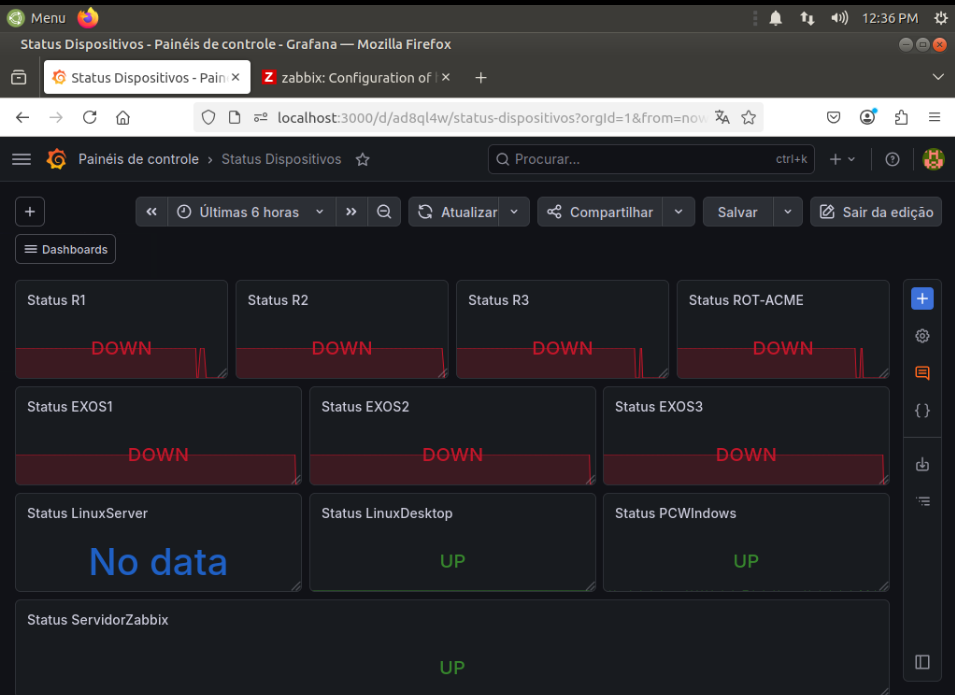
\includegraphics[width=\linewidth,height=10cm]{fig/zabbix/dash1.png}
    \caption{Dashboard de monitoramento do status dos dispositivos da rede.}
    \label{fig:dashStatus}
\end{figure*}


Além disso, nesse dashboard foi adicionado um menu suspenso contendo links para os demais dashboards configurados no Grafana, facilitando a navegação entre as diferentes telas de monitoramento, conforme mostrado na Figura~\ref{fig:dashDropdown}.

\begin{figure}[H]
    \centering
    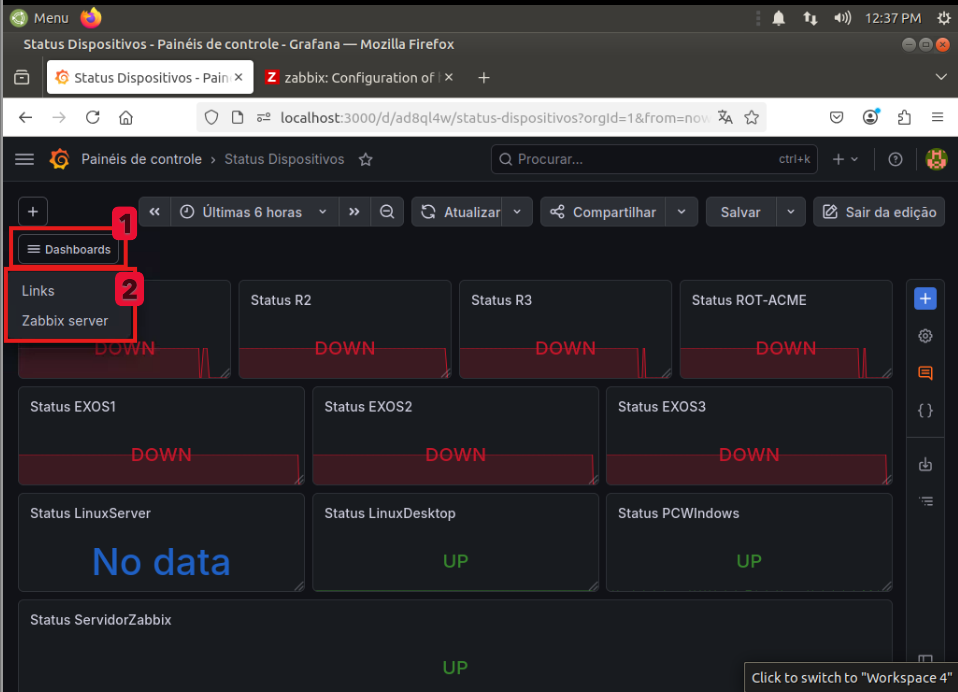
\includegraphics[width=1\linewidth]{fig/zabbix/dash2.png}
    \caption{Menu suspenso contendo links para navegação entre os dashboards: 1. Menu Dashboard; 2. Links para os dashboards disponíveis.}
    \label{fig:dashDropdown}
\end{figure}

O dashboard apresentado na Figura~\ref{fig:dashLinks} foi desenvolvido para o monitoramento das interfaces de rede dos roteadores e switches. Nesse painel, é possível verificar a atividade dos dispositivos e o estado operacional de cada interface ou porta monitorada, permitindo identificar problemas de conectividade e falhas nos enlaces da rede.

\begin{figure*}[t]
    \centering
    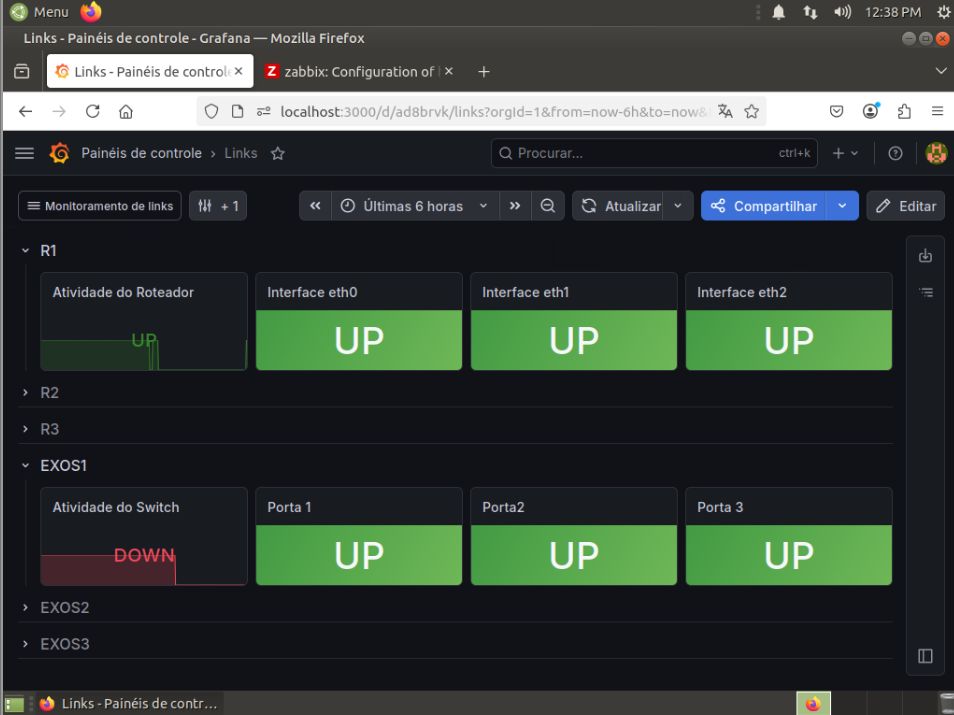
\includegraphics[width=\linewidth,height=10cm]{fig/zabbix/dash3.png}
    \caption{Dashboard de monitoramento das interfaces de roteadores e switches.}
    \label{fig:dashLinks}
\end{figure*}

Por fim, o dashboard da Figura~\ref{fig:dashServidor} apresenta informações relacionadas ao servidor Zabbix. Nesse painel, foram configurados indicadores de status do servidor, utilização de disco, uso de memória RAM, utilização de CPU, carga do sistema e monitoramento da interface de rede, fornecendo uma visão geral do desempenho do servidor responsável pelo monitoramento da infraestrutura.

\begin{figure*}[t]
    \centering
    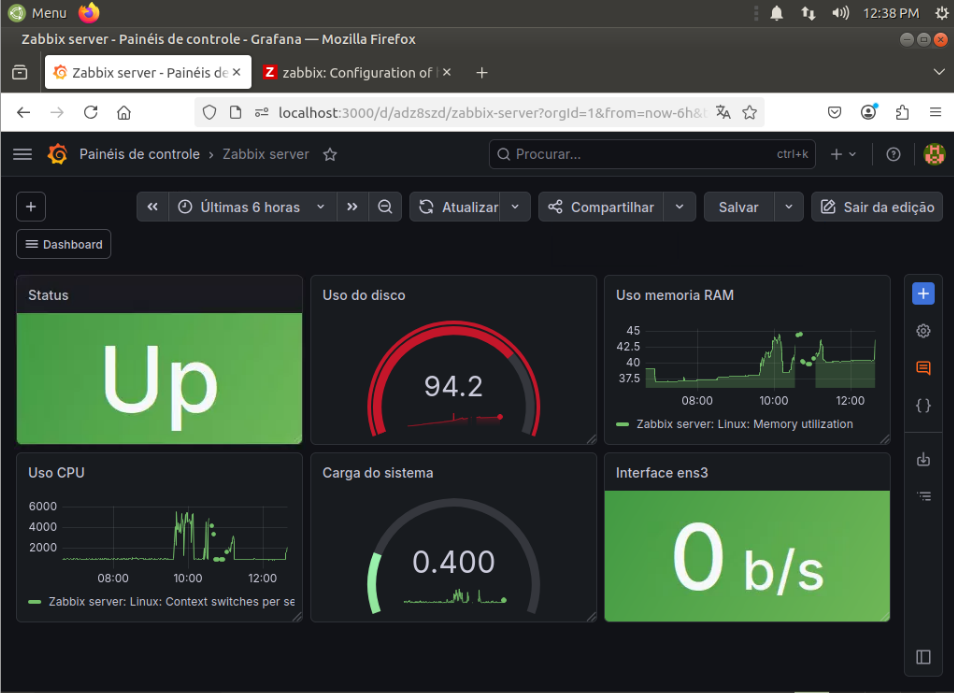
\includegraphics[width=\linewidth,height=10cm]{fig/zabbix/dash4.png}
    \caption{Dashboard de monitoramento do servidor Zabbix.}
    \label{fig:dashServidor}
\end{figure*}